\section{Muon Momentum Resolution}

by travelling in Iron, High-Pt muons ($P_{t}>200GeV$) suffer from high energy
loss due to radiative processes. The transverse momentum measurement relays on
sagita ($s \propto 1/Pt$) which is associated with the number of hits found on
the Tracker and the Muon subsystems. As the number of hits is lower on the so called
tracker muons, i.e muons that were reconstructed from hits in the tracker and the
first station of the muon sistem, a study is needed to determine
the resolution of this Pt measurement for \verb|trackerHighPt| ID muons.


From MC simulations it is possible to access the true momenta of the muons and
a comparison with the reconstructed momentum can be given in terms of the
residual momentum:

\begin{equation}
  \frac{P_{GEN}}{P_{RECO}} - 1 = \frac{\dfrac{1}{P_{RECO}}-\dfrac{1}{P_{GEN}}}{\dfrac{1}{P_{RECO}}}
\end{equation}

The resolution can be extracted by fitting the event profile with a
Double-Sided Crystal Ball (DSCB) distribution which consists of three diferent regions:
a gaussian center described by a mean $\mu$ and standard deviation $\sigma$ with two
exponential tails modelling the effects of radiative processes in the detector.
The two tails are controlled by four parameters, $n_{L}$ and $\alpha_{L}$ for the
left tail and $n_{R}$ and $\alpha_{R}$ for the right tail. $\alpha$ describes how
far away (as a factor of $sigma$) from the gaussian mean the exponential decay
intersects the guassian core, while $n$ controls the growth (decay) of the
left (right) exponential tail.

\begin{figure}[tph]
  \centering
  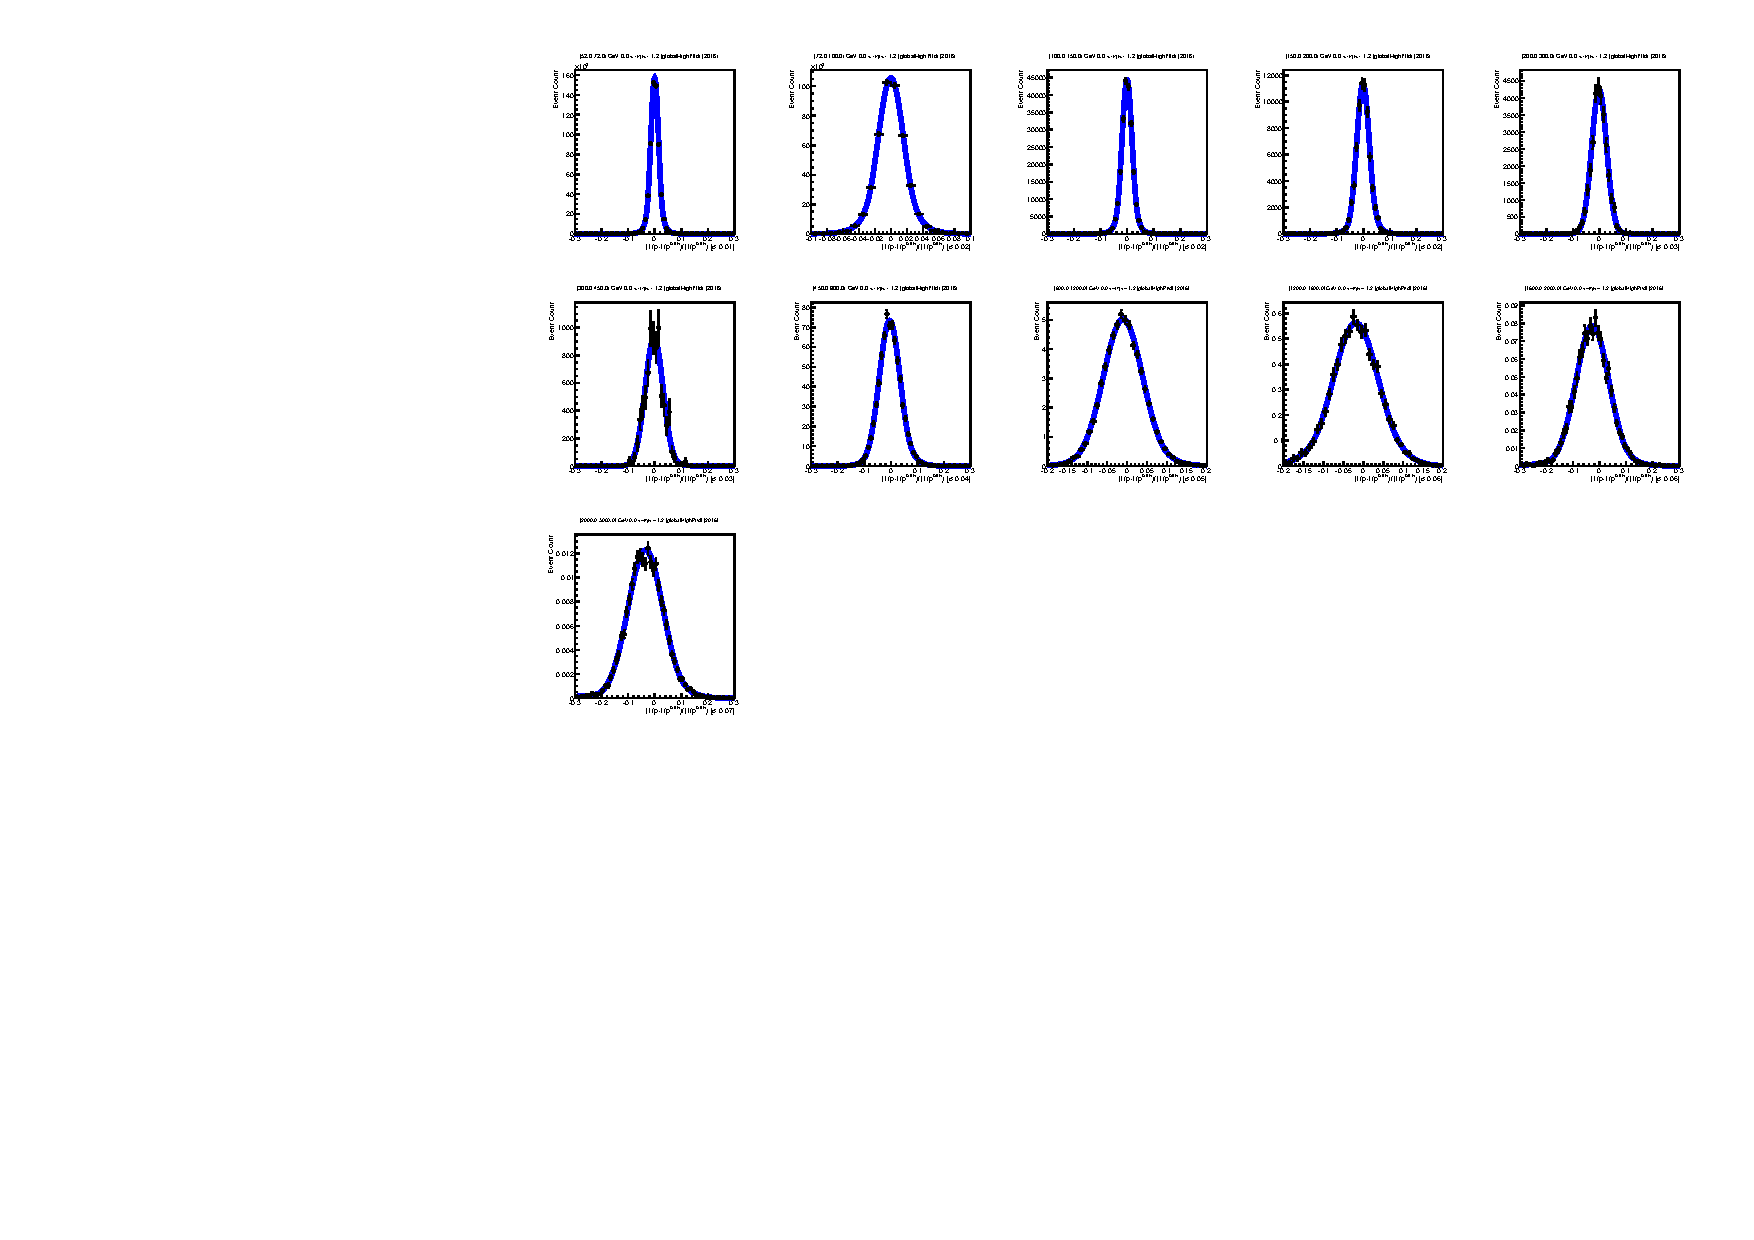
\includegraphics[width=.9\textwidth]{fig/MomentumResolution/2016_HPResB_G_.pdf}
  \caption{Residual momentum for different transverse momentum bins
    or \texttt{globalHighPt} muons in the muon barrel $(0.0<\eta<1.2)$.
    The double-sided crystal ball fit is shown with a blue solid line,
    the number of events as counted from MC samples are shown in black markers.
    The width $(\sigma)$ of the gaussian portion of the distribution is
    shown on the bottom label, it shows evidence of how the resolution
    increases as the momentum range gets higher.}
  \label{fig:MomentumResolutionBins_Barrel_Global}
\end{figure}

\begin{figure}[tph]
  \centering
  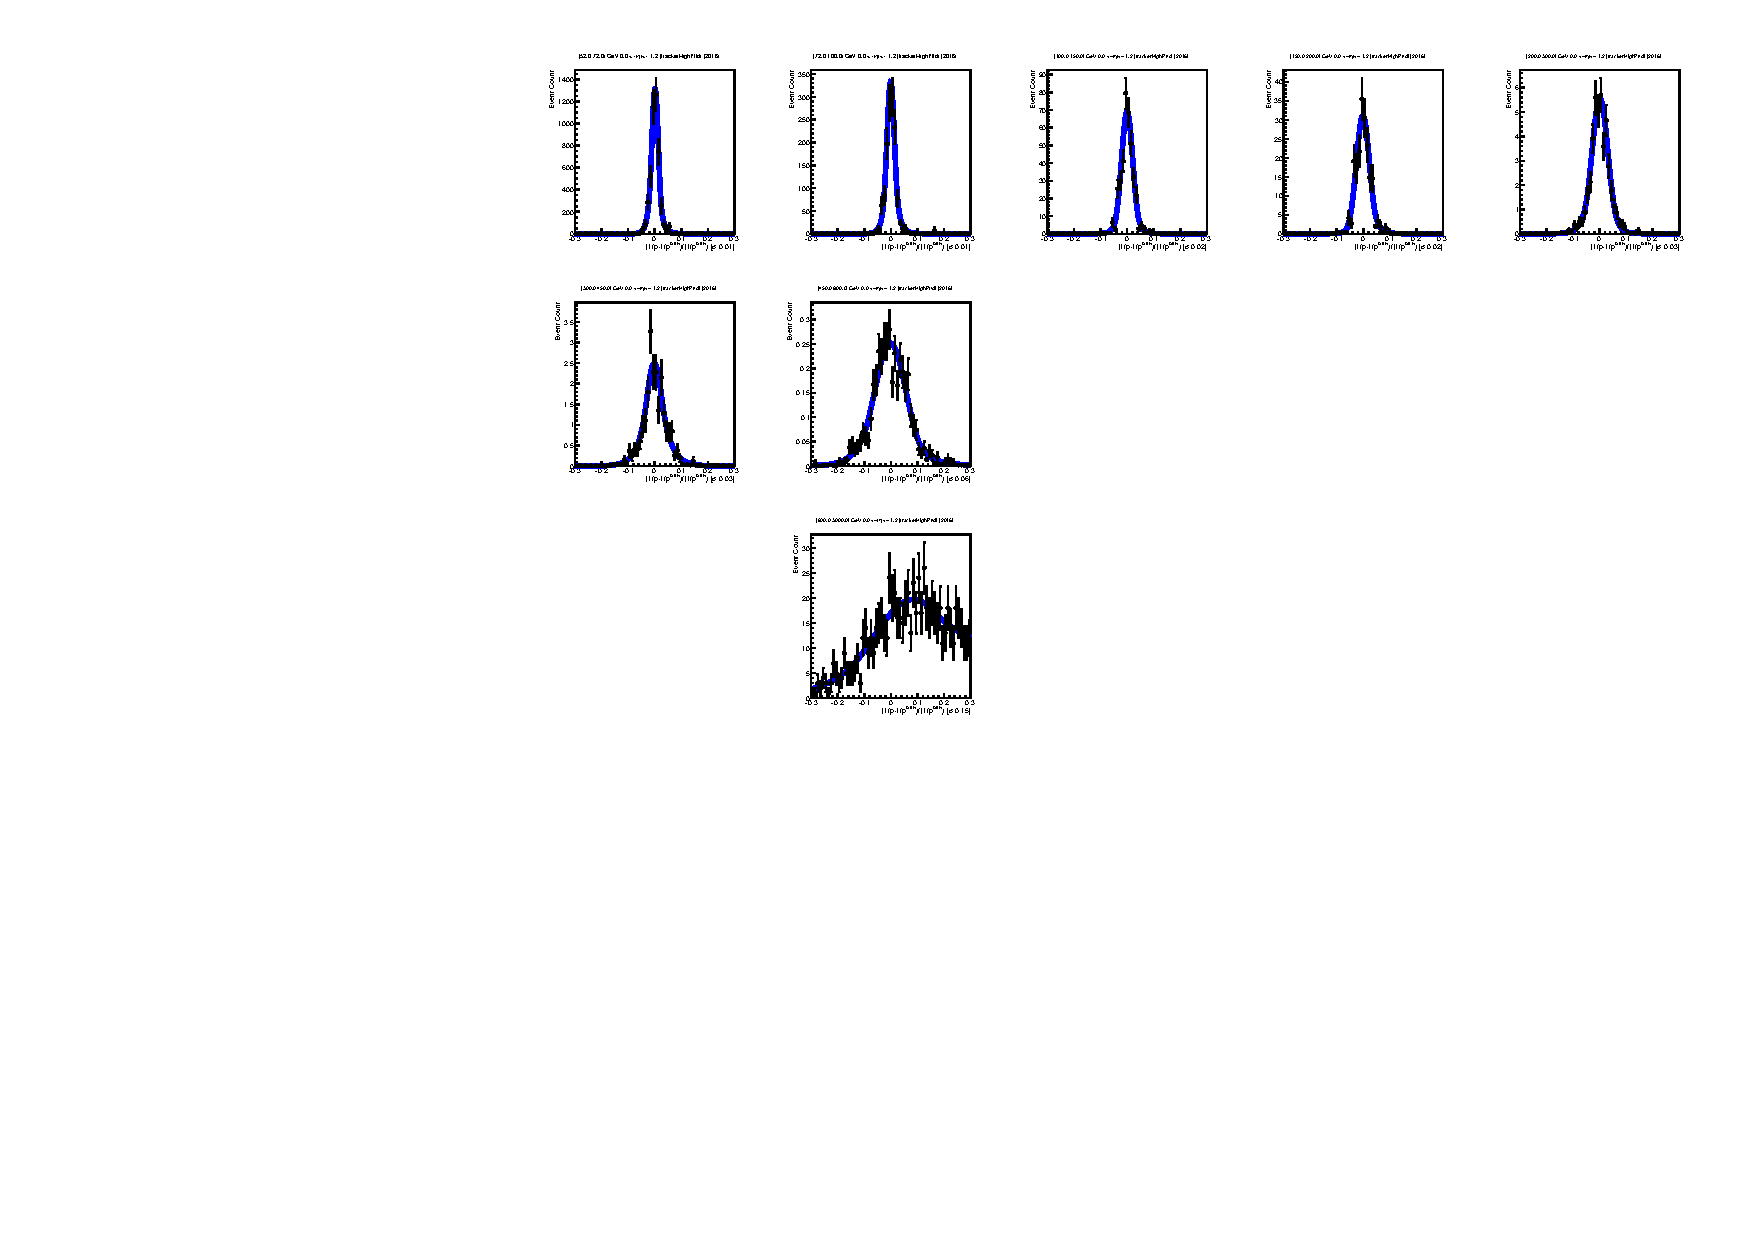
\includegraphics[width=.9\textwidth]{fig/MomentumResolution/2016_HPResB_T_.pdf}
  \caption{Residual momentum for different transverse momentum bins
    for \texttt{trackerHighPt} muons in the muon barrel $(0.0<\eta<1.2)$.
    The double-sided crystal ball fit is shown with a blue solid line,
    the width $(\sigma)$ of the gaussian portion of the distribution is
    shown on the bottom label.}
  \label{fig:MomentumResolutionBins_Barrel_Tracker}
\end{figure}

\begin{figure}[tph]
  \centering
  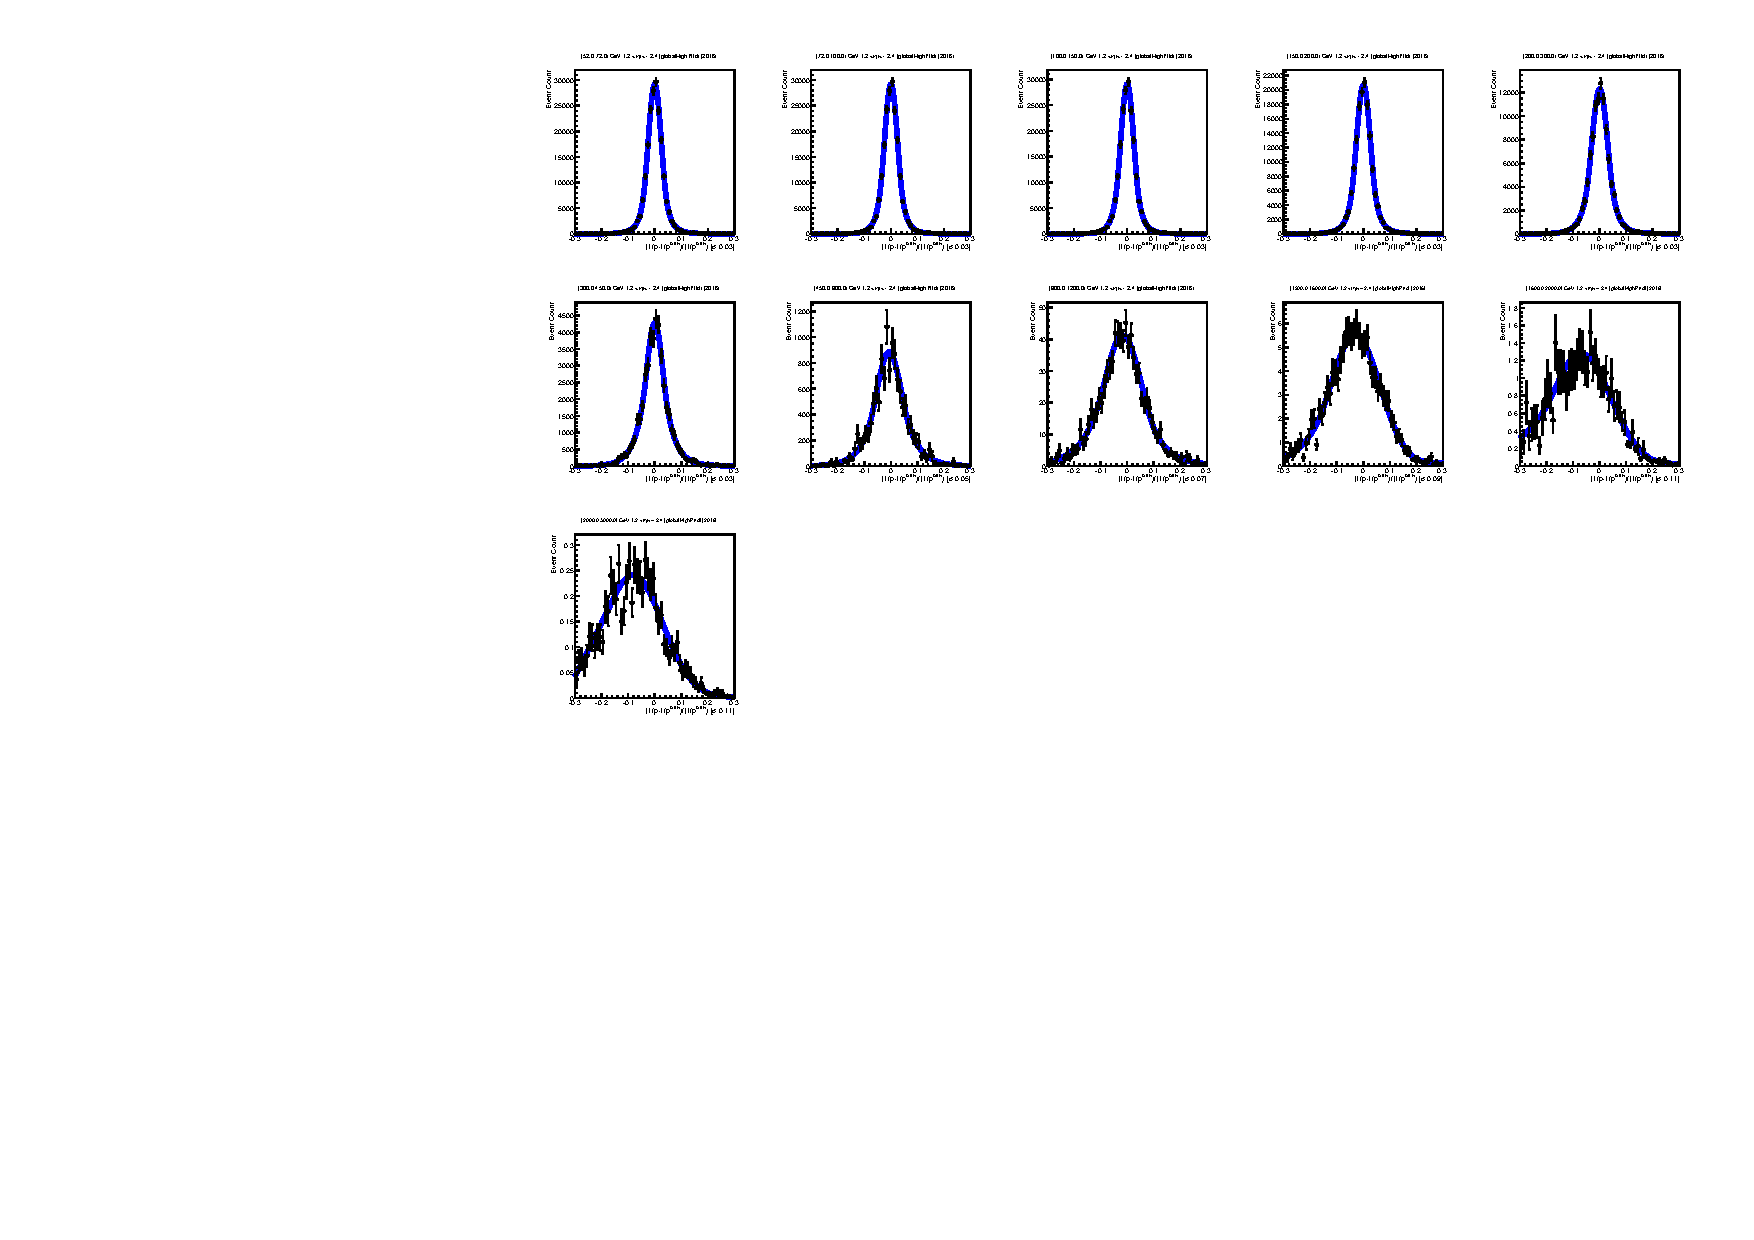
\includegraphics[width=.9\textwidth]{fig/MomentumResolution/2016_HPResE_G_.pdf}
  \caption{Residual momentum for different transverse momentum bins
    or \texttt{globalHighPt} muons in the muon endcap $(1.2<\eta<2.4)$.
    The double-sided crystal ball fit is shown with a blue solid line,
    the number of events as counted from MC samples are shown in black markers.
    The width $(\sigma)$ of the gaussian portion of the distribution is
    shown on the bottom label.}
  \label{fig:MomentumResolutionBins_Endcap_Global}
\end{figure}

\begin{figure}[tph]
  \centering
  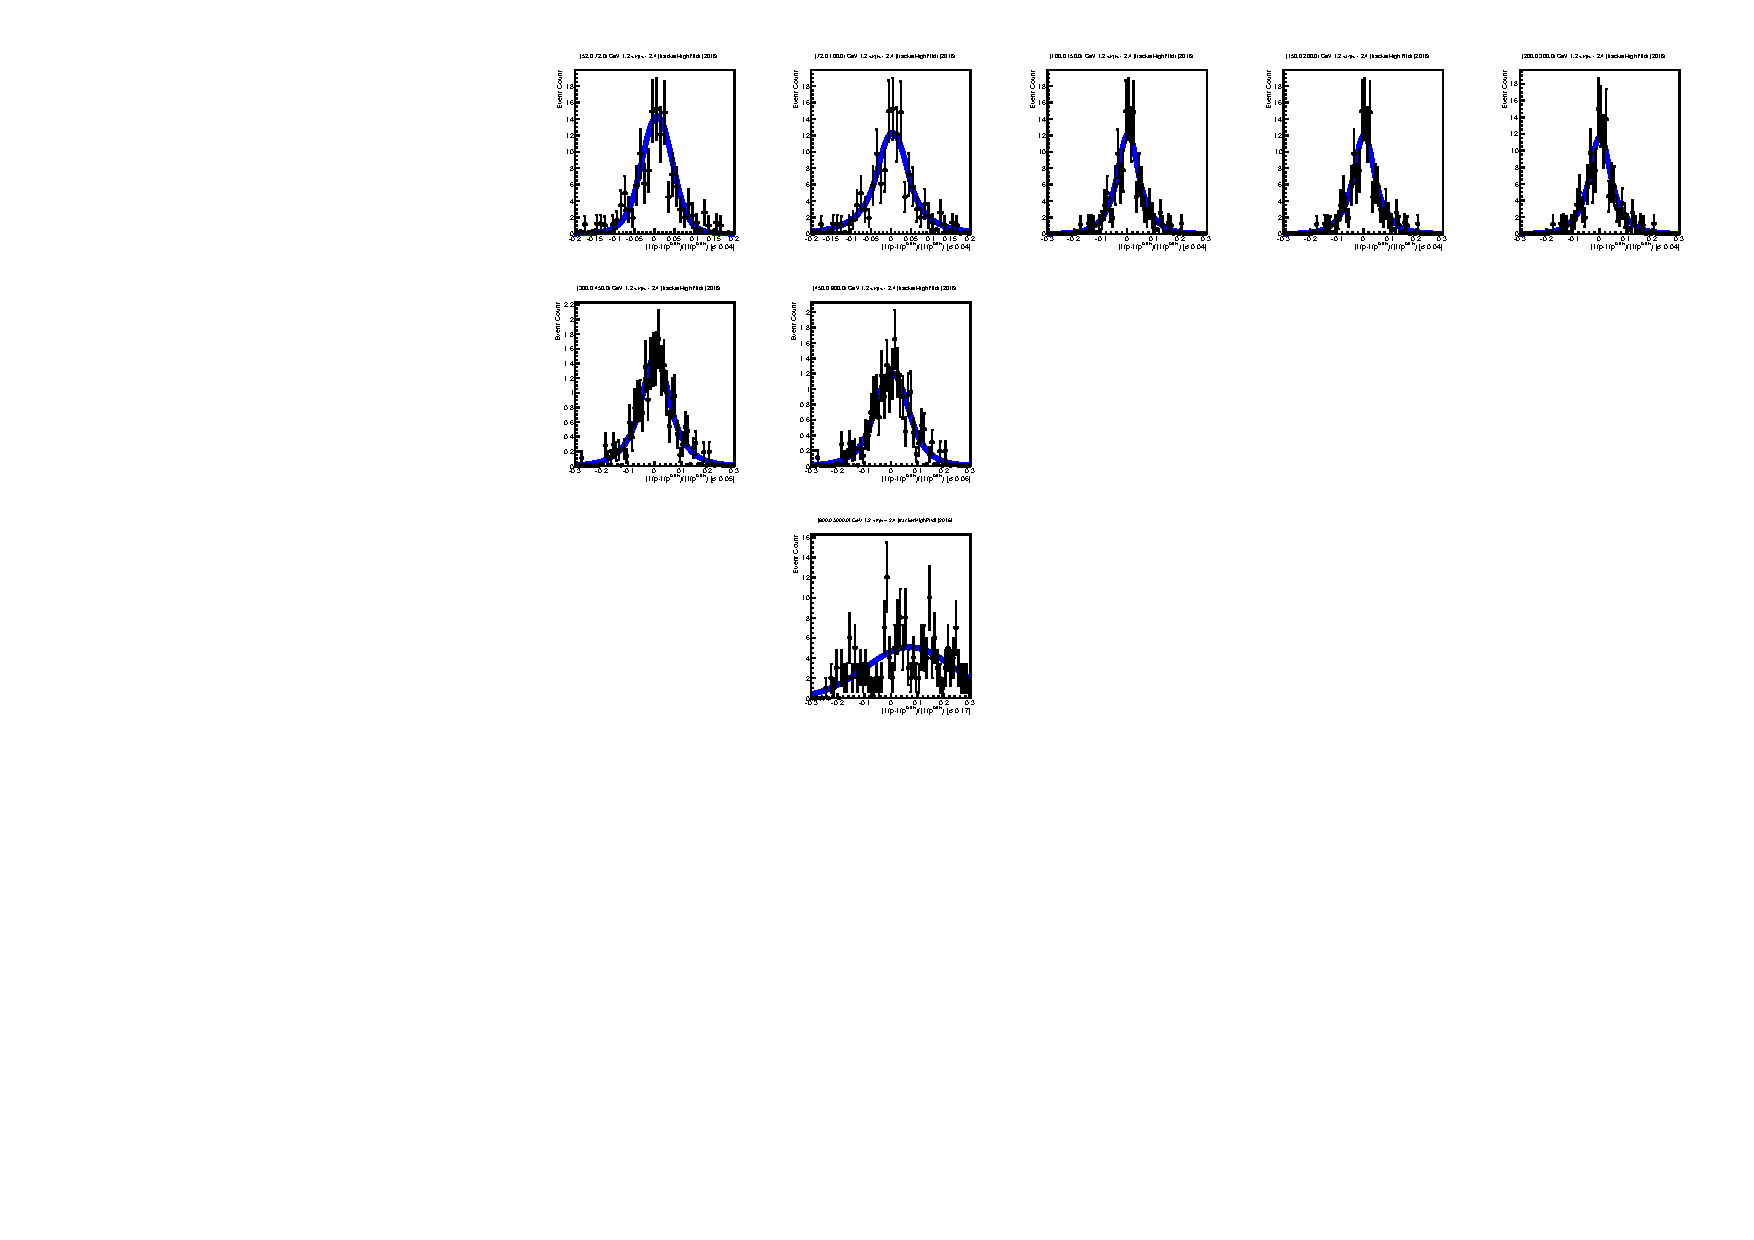
\includegraphics[width=.9\textwidth]{fig/MomentumResolution/2016_HPResE_T_.pdf}
  \caption{Residual momentum for different transverse momentum bins
    for \texttt{trackerHighPt} muons in the muon endcap $(1.2<\eta<2.4)$.
    The double-sided crystal ball fit is shown with a blue solid line,
    the width $(\sigma)$ of the gaussian portion of the distribution is
    shown on the bottom label.}
  \label{fig:MomentumResolutionBins_Endcap_Tracker}
\end{figure}


\begin{figure}[tph]
  \centering
  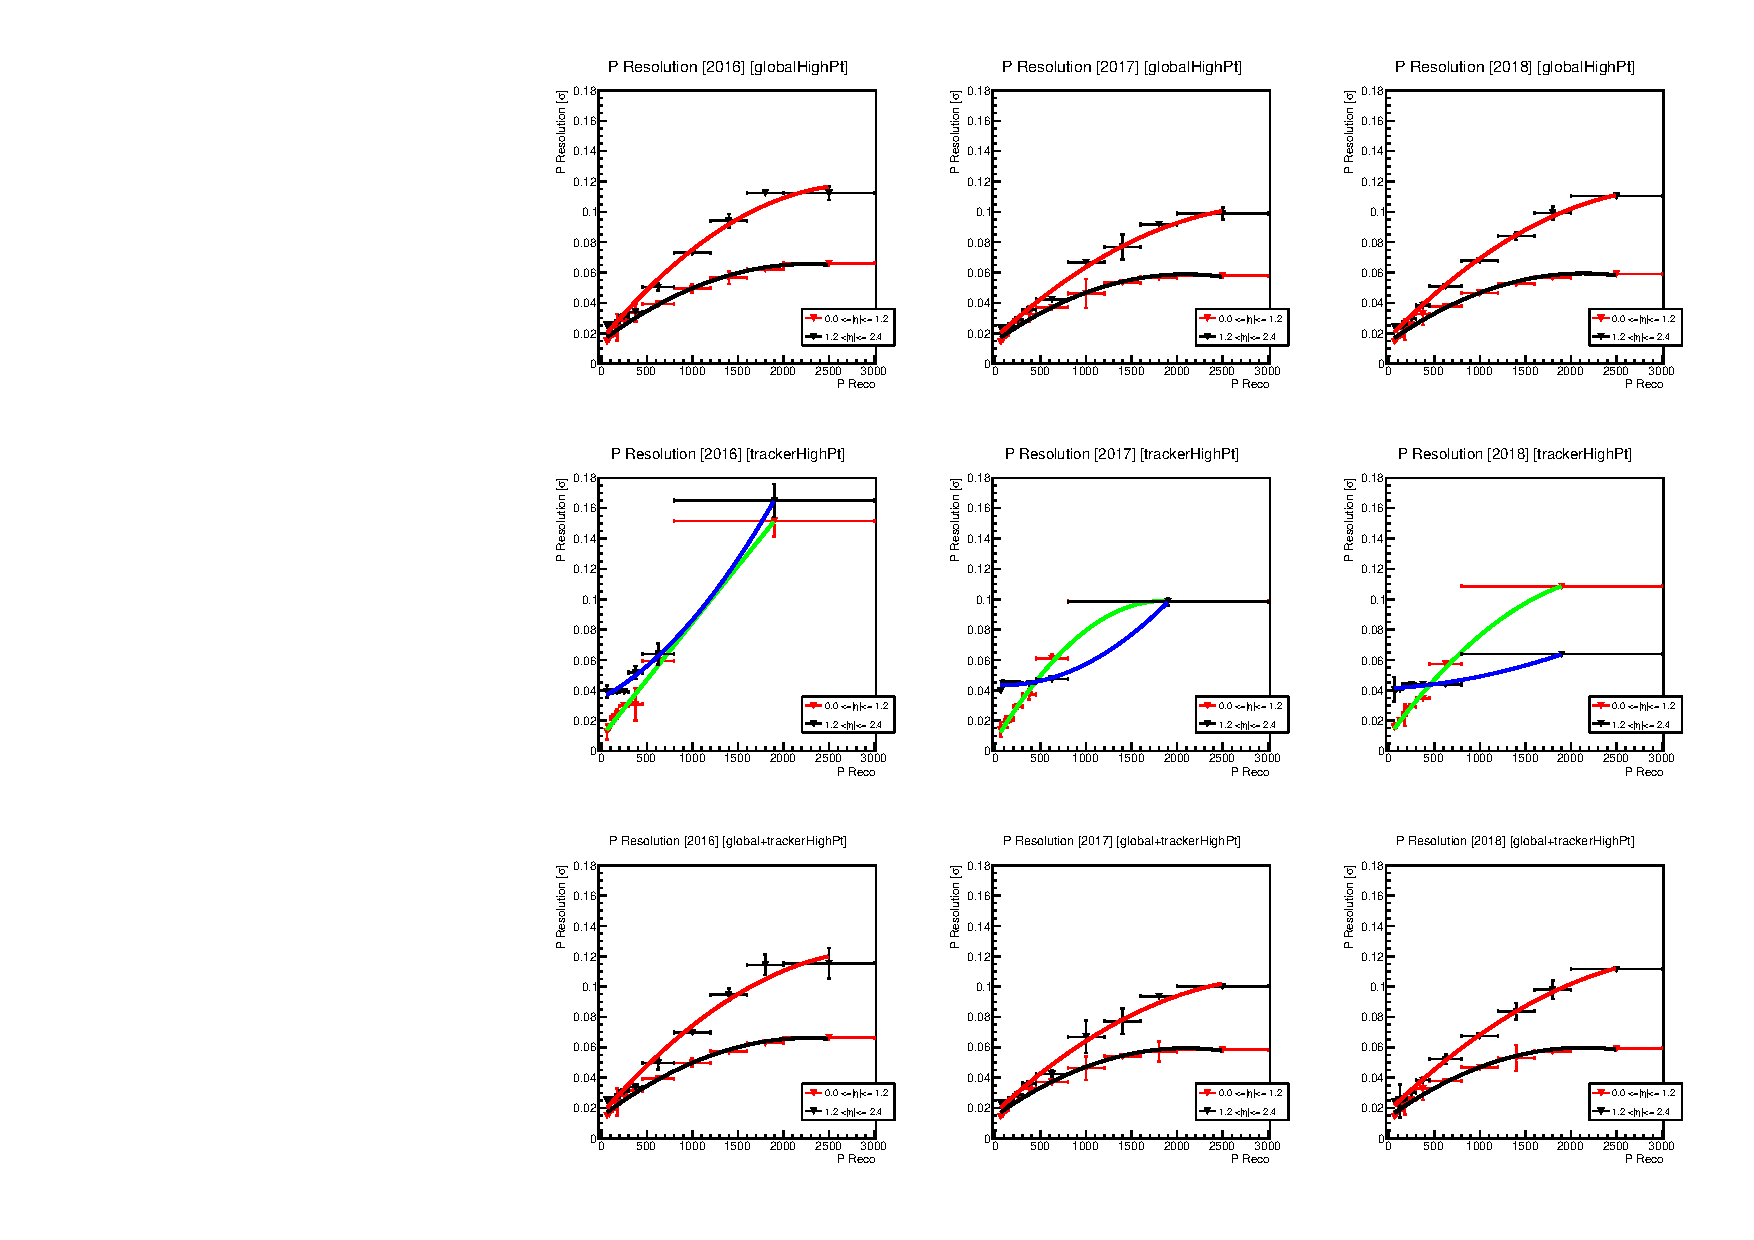
\includegraphics[width=.9\textwidth]{fig/MomentumResolution/ResolutionMeasurement.pdf}
  \caption{Momentum resolution for Run II. A second degree polynomial shown in
    colored solid lines is used to fit the momentum resolution as a function of
    the reconstructed momentum.}
  \label{fig:ResolutionMeasurement}
\end{figure}


\begin{sidewaystable}[htb]
\begin{center}
  \caption{Montecarlo Samples used to study the Muon Momentum Resolution}
\footnotesize
\begin{tabular}{|l|l|l|}
\hline
Year & Sample & XSec [pb] \\ \hline
\hline
2016 & ZToMuMu\_NNPDF30\_13TeV-powheg\_M\_50\_120 & 2.116e+03\\
&ZToMuMu\_NNPDF30\_13TeV-powheg\_M\_120\_200 & 2.058e+01\\
&ZToMuMu\_NNPDF30\_13TeV-powheg\_M\_200\_400 & 2.890e+00\\
&ZToMuMu\_NNPDF30\_13TeV-powheg\_M\_400\_800 & 2.515e-01\\
&ZToMuMu\_NNPDF30\_13TeV-powheg\_M\_800\_1400 & 1.709e-02\\
&ZToMuMu\_NNPDF30\_13TeV-powheg\_M\_1400\_2300 & 1.370e-03\\
&ZToMuMu\_NNPDF30\_13TeV-powheg\_M\_2300\_3500 & 8.282e-05\\
&ZToMuMu\_NNPDF30\_13TeV-powheg\_M\_3500\_4500 & 3.414e-06\\
&ZToMuMu\_NNPDF30\_13TeV-powheg\_M\_4500\_6000 & 3.650e-07\\
&ZToMuMu\_NNPDF30\_13TeV-powheg\_M\_6000\_Inf & 2.526e-08\\
\hline
2017 & ZToMuMu\_NNPDF31\_TuneCP5\_13TeV-powheg-pythia8\_M\_50\_120 & 2.116e+03\\
&ZToMuMu\_NNPDF31\_TuneCP5\_13TeV-powheg-pythia8\_M\_120\_200 & 2.058e+01\\
&ZToMuMu\_NNPDF31\_TuneCP5\_13TeV-powheg-pythia8\_M\_200\_400 & 2.890e+00\\
&ZToMuMu\_NNPDF31\_TuneCP5\_13TeV-powheg-pythia8\_M\_400\_800 & 2.515e-01\\
&ZToMuMu\_NNPDF31\_TuneCP5\_13TeV-powheg-pythia8\_M\_800\_1400 & 1.709e-02\\
&ZToMuMu\_NNPDF31\_TuneCP5\_13TeV-powheg-pythia8\_M\_1400\_2300 & 1.370e-03\\
&ZToMuMu\_NNPDF31\_TuneCP5\_13TeV-powheg-pythia8\_M\_2300\_3500 & 8.282e-05\\
&ZToMuMu\_NNPDF31\_TuneCP5\_13TeV-powheg-pythia8\_M\_3500\_4500 & 3.414e-06\\
&ZToMuMu\_NNPDF31\_TuneCP5\_13TeV-powheg-pythia8\_M\_4500\_6000 & 3.650e-07\\
&ZToMuMu\_NNPDF31\_TuneCP5\_13TeV-powheg-pythia8\_M\_6000\_Inf & 2.526e-08\\
\hline
2018 & ZToMuMu\_NNPDF31\_TuneCP5\_13TeV-powheg-pythia8\_M\_50\_120 & 2.116e+03\\
&ZToMuMu\_NNPDF31\_TuneCP5\_13TeV-powheg-pythia8\_M\_120\_200 & 2.058e+01\\
&ZToMuMu\_NNPDF31\_TuneCP5\_13TeV-powheg-pythia8\_M\_200\_400 & 2.890e+00\\
&ZToMuMu\_NNPDF31\_TuneCP5\_13TeV-powheg-pythia8\_M\_400\_800 & 2.515e-01\\
&ZToMuMu\_NNPDF31\_TuneCP5\_13TeV-powheg-pythia8\_M\_800\_1400 & 1.709e-02\\
&ZToMuMu\_NNPDF31\_TuneCP5\_13TeV-powheg-pythia8\_M\_1400\_2300 & 1.370e-03\\
&ZToMuMu\_NNPDF31\_TuneCP5\_13TeV-powheg-pythia8\_M\_2300\_3500 & 8.282e-05\\
&ZToMuMu\_NNPDF31\_TuneCP5\_13TeV-powheg-pythia8\_M\_3500\_4500 & 3.414e-06\\
&ZToMuMu\_NNPDF31\_TuneCP5\_13TeV-powheg-pythia8\_M\_4500\_6000 & 3.650e-07\\
&ZToMuMu\_NNPDF31\_TuneCP5\_13TeV-powheg-pythia8\_M\_6000\_Inf & 2.526e-08\\
\hline
\end{tabular}
\label{tab:MomentumResolutionSamples}
\end{center}
\end{sidewaystable}

These studies were performed by simulating the standard model Z boson production
decaying to a pair of Muons ($Z\rightarrow\mu\mu$) the complete list of samples is
provided on table \ref{tab:MomentumResolutionSamples}.
Z-Mass binned samples were used in order to increase the number of available
statistics in a wide range of transverse momentum, specially on the High-Pt sector.

\begin{figure}[tph]
  \centering
  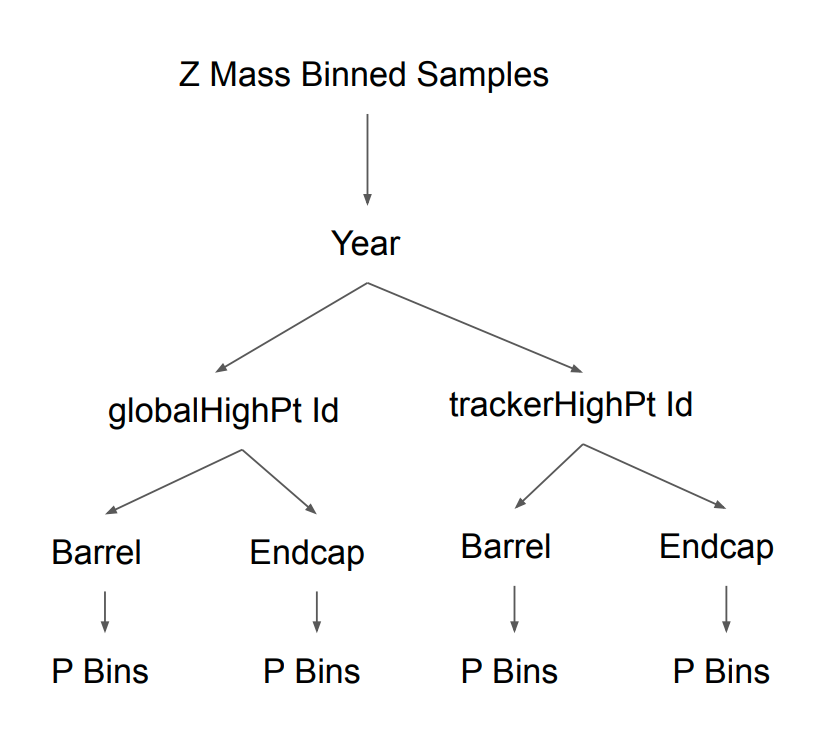
\includegraphics[width=.5\textwidth]{fig/MomentumResolution/MomentumResolutionBins.png}
  \caption{Signal efficiency for individual and combined High Level Triggers for Run II}
  \label{fig:MomentumResolutionBins}
\end{figure}


A counting experiment following the trigger and muon selection described on
section %\ref{}%
collects the momentum resolution for each indivual muon which is then classified
in different bins depending on their ID, either global or tracker High-Pt; the $\eta$
region in the Muon detector, i.e the barrel ($\lvert eta\lvert< 1.2$) or
the endcap ($1.2 < \lvert eta \lvert < 2.4$); and its transverse momentum range
(see figure \ref{fig:MomentumResolutionBins}).

A fit is performed on the distribution by using a Double-Sided Crystall Ball (DSCB)
(\verb|RooCrystalBall| in \verb|RooFit|)
The width of the gaussian portion of the DSCB provides the
resolution (as a percentage) while the mean accounts for any bias present on the
momentum measurements. Distributions with their fits are shown for \verb|globalHighPt|
within the muon barrel on figure \ref{fig:MomentumResolutionBins_Barrel_Global}, the muon
endcap on figure \ref{fig:MomentumResolutionBins_Endcap_Global};
and \verb|trackerHighPt| muons on the barrel
(figure \ref{fig:MomentumResolutionBins_Barrel_Tracker})
and the endcap (figure \ref{fig:MomentumResolutionBins_Endcap_Tracker}).
The results from the fits are shown in figure \ref{fig:ResolutionMeasurement}.

As shown by figures \ref{fig:MomentumResolutionBins_Barrel_Global} and
\ref{fig:MomentumResolutionBins_Barrel_Tracker} the amount of statistics
available for \verb|globalHighPt| muons is greater than for
\verb|trackerHighPt| muons. 

\subsection{Z-Mass Resolution}

\begin{sidewaystable}[htb]
\begin{center}
  \caption{Montecarlo Samples for Z Mass Resolution studies}
\footnotesize
\begin{tabular}{|l|l|l|}
\hline
Year & Sample & XSec [pb] \\ \hline
\hline
2016 & DYJetsToMuMu\_M-50\_Zpt-150toInf\_TuneCP5\_13TeV-madgraphMLM\_pdfwgt\_F-pythia8 & 6.178e+00\\
\hline
2017 & DYJetsToMuMu\_M-50\_Zpt-150toInf\_TuneCP5\_13TeV-madgraphMLM\_pdfwgt\_F-pythia8 & 6.182e+00\\
\hline
2018 & DYJetsToMuMu\_M-50\_Zpt-150toInf\_TuneCP5\_13TeV-madgraphMLM\_pdfwgt\_F-pythia8 & 6.178e+00\\
\hline
\end{tabular}
\label{tab:ZMassResolutionSamples}
\end{center}
\end{sidewaystable}

\begin{figure}[tph]
  \centering
  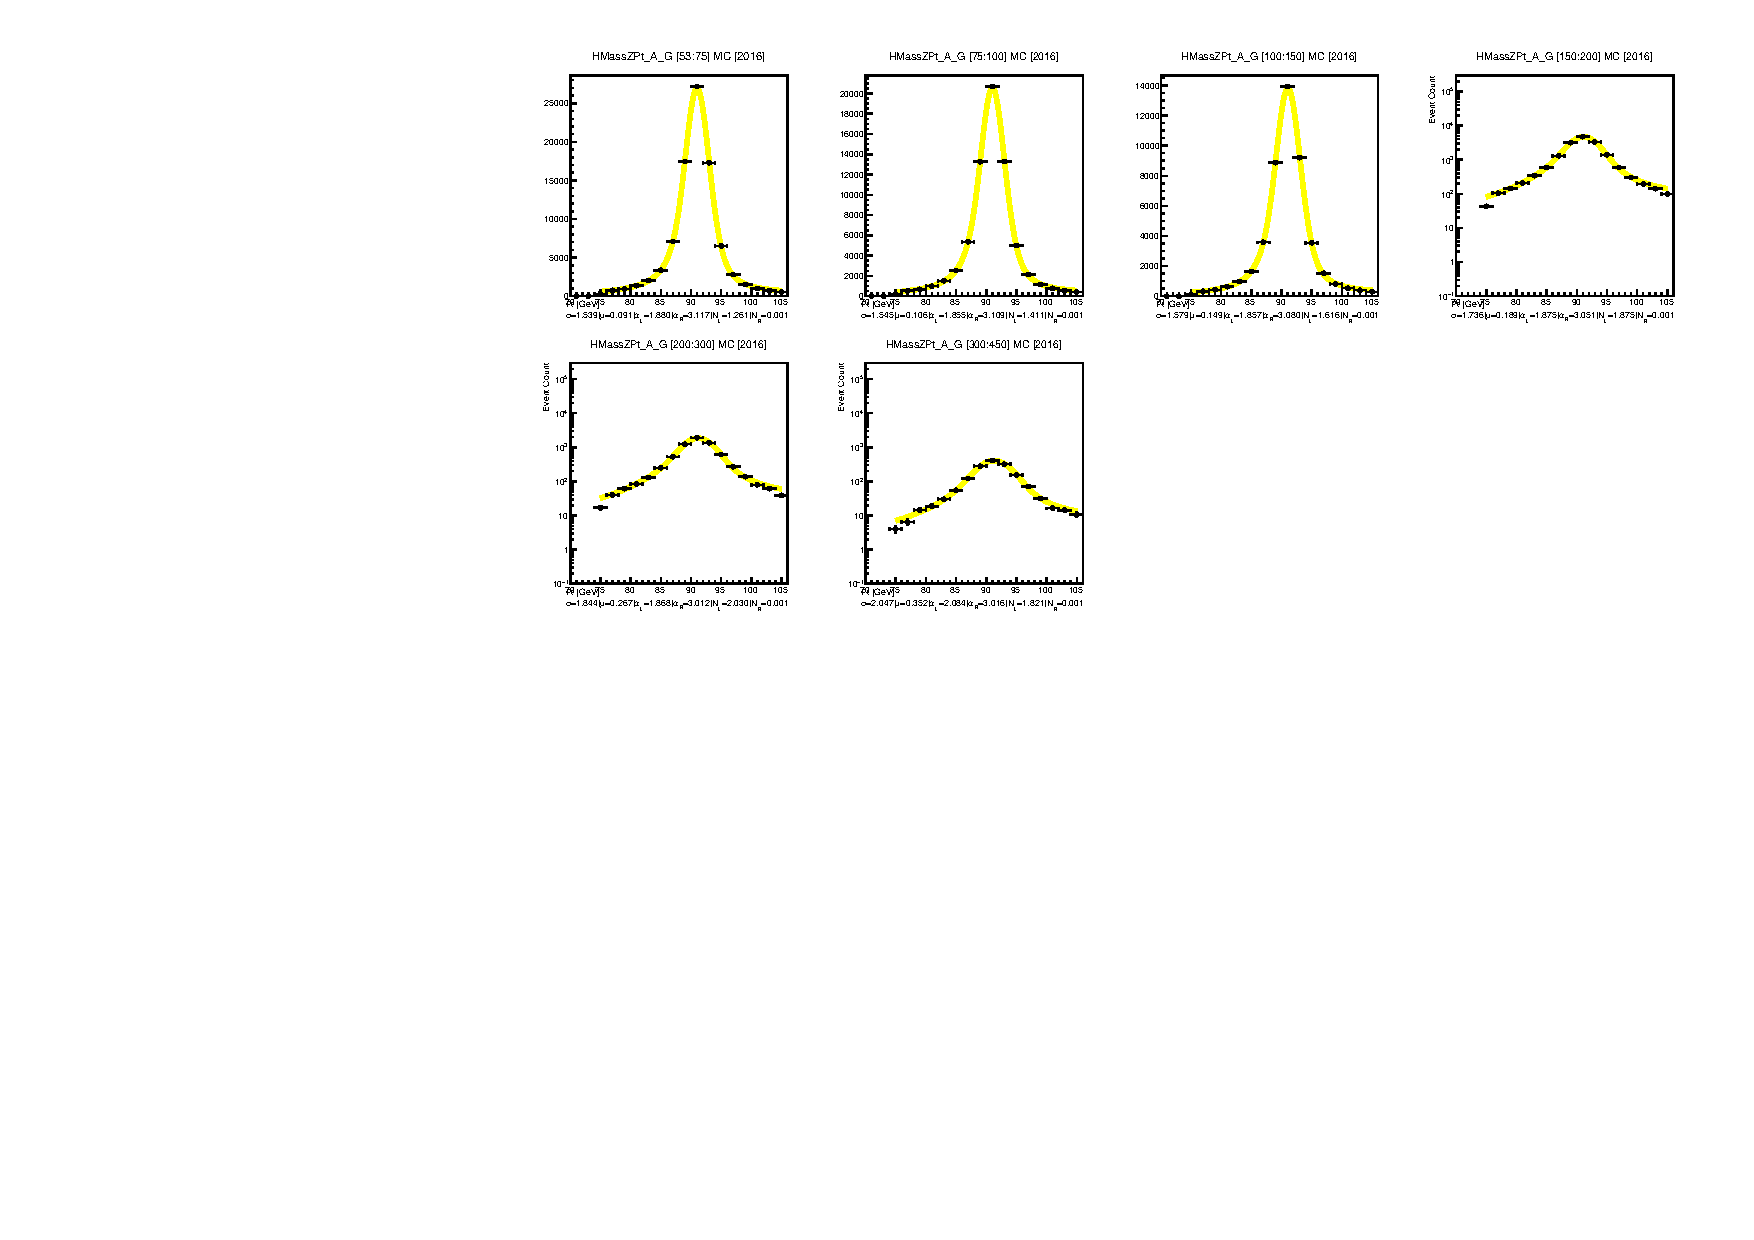
\includegraphics[width=.9\textwidth]{fig/MomentumResolution/2016_ZPeakResoultion_G_Fits_MC.pdf}
  \caption{Dimuon mass resolution for different transverse momentum bins from MC
    simulation for \texttt{globalHighPt} muons. The Breit-Wigner convoluted with the
    double-sided crystal ball fit is shown in solid yellow line and parameters
    of the fit are shown on the bottom of each plot.}
  \label{fig:ZMassResolution_MC_Global}
\end{figure}

\begin{figure}[tph]
  \centering
  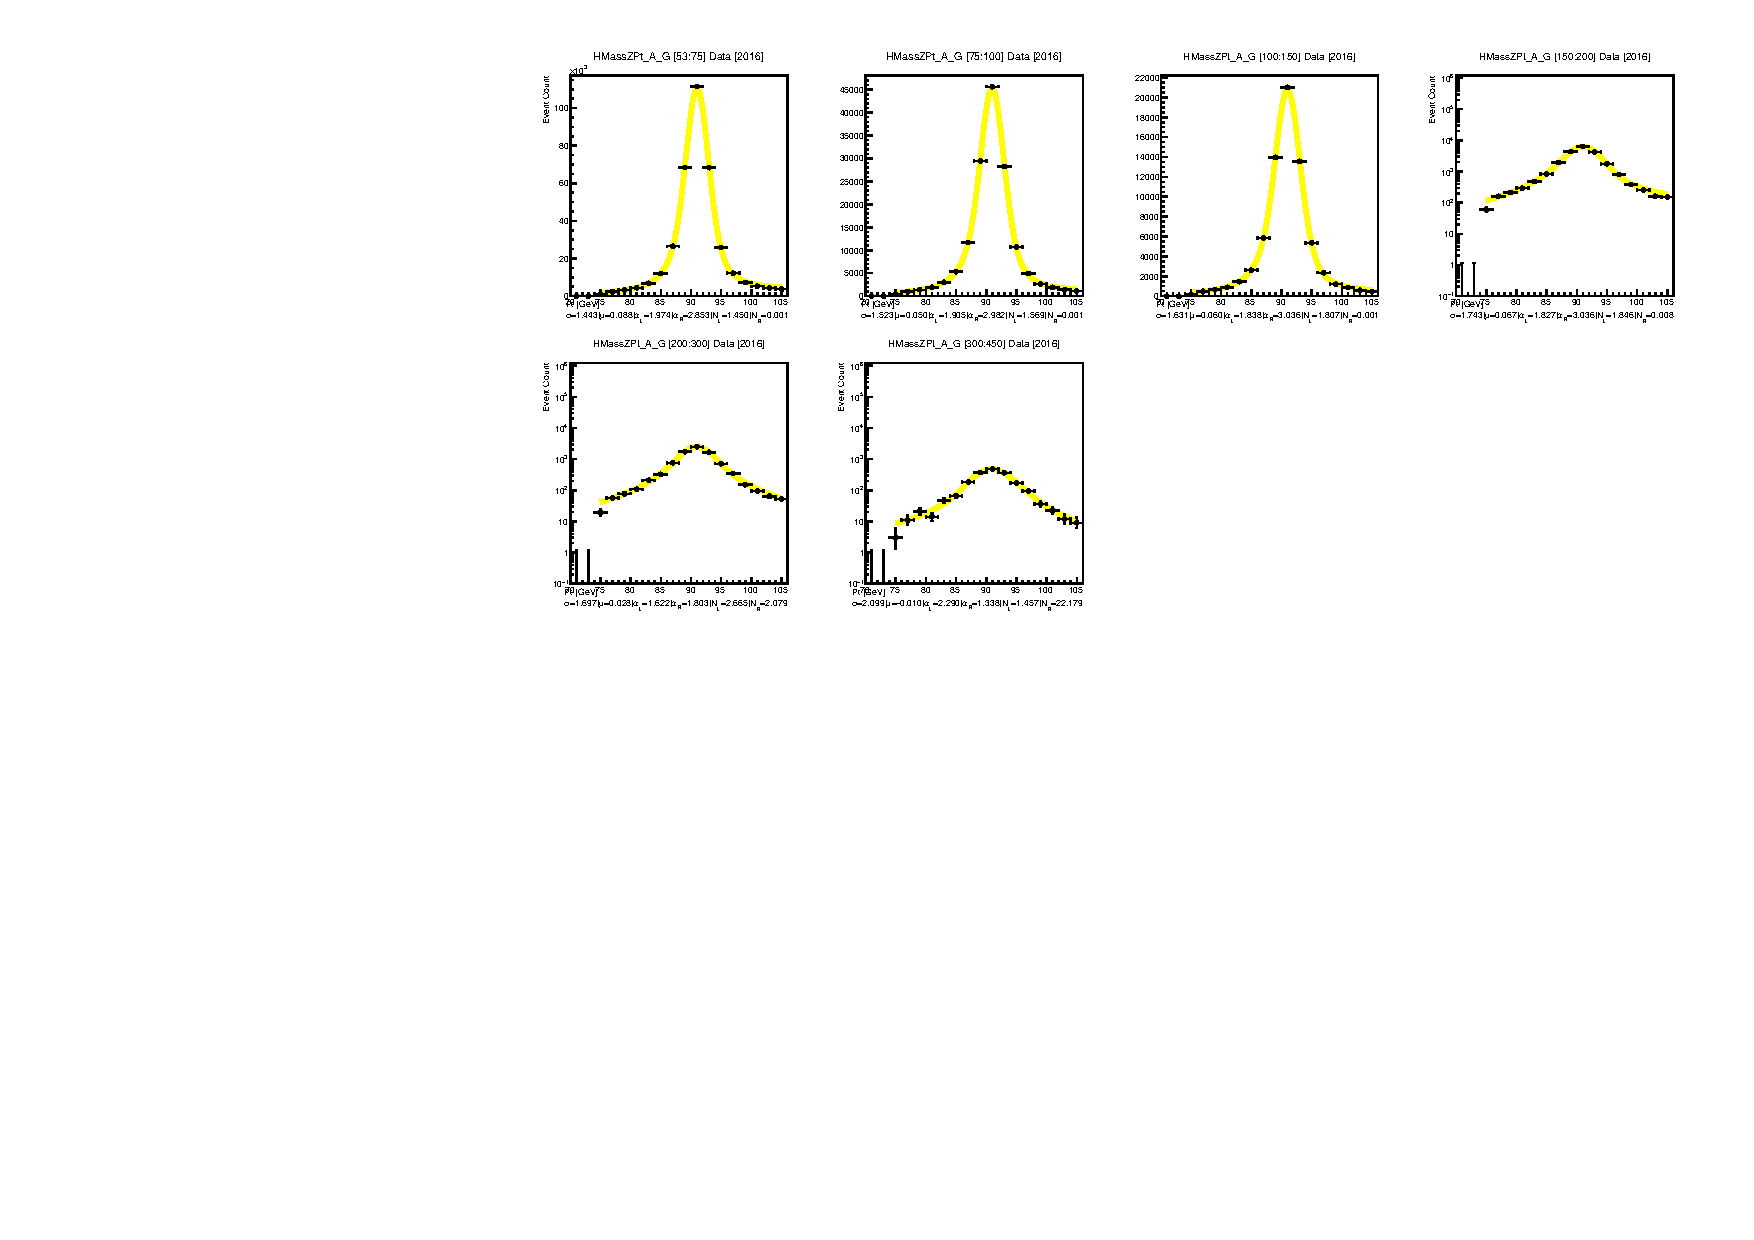
\includegraphics[width=.9\textwidth]{fig/MomentumResolution/2016_ZPeakResolution_G_Fits_Data.pdf}
  \caption{Dimuon mass resolution for different transverse momentum bins from 2016
    Data for \texttt{globalHighPt} muons. The Breit-Wigner convoluted with the
    double-sided crystal ball fit is shown in solid yellow line and parameters
    of the fit are shown on the bottom of each plot.}
  \label{fig:ZMassResolution_Data_Global}
\end{figure}

\begin{figure}[tph]
  \centering
  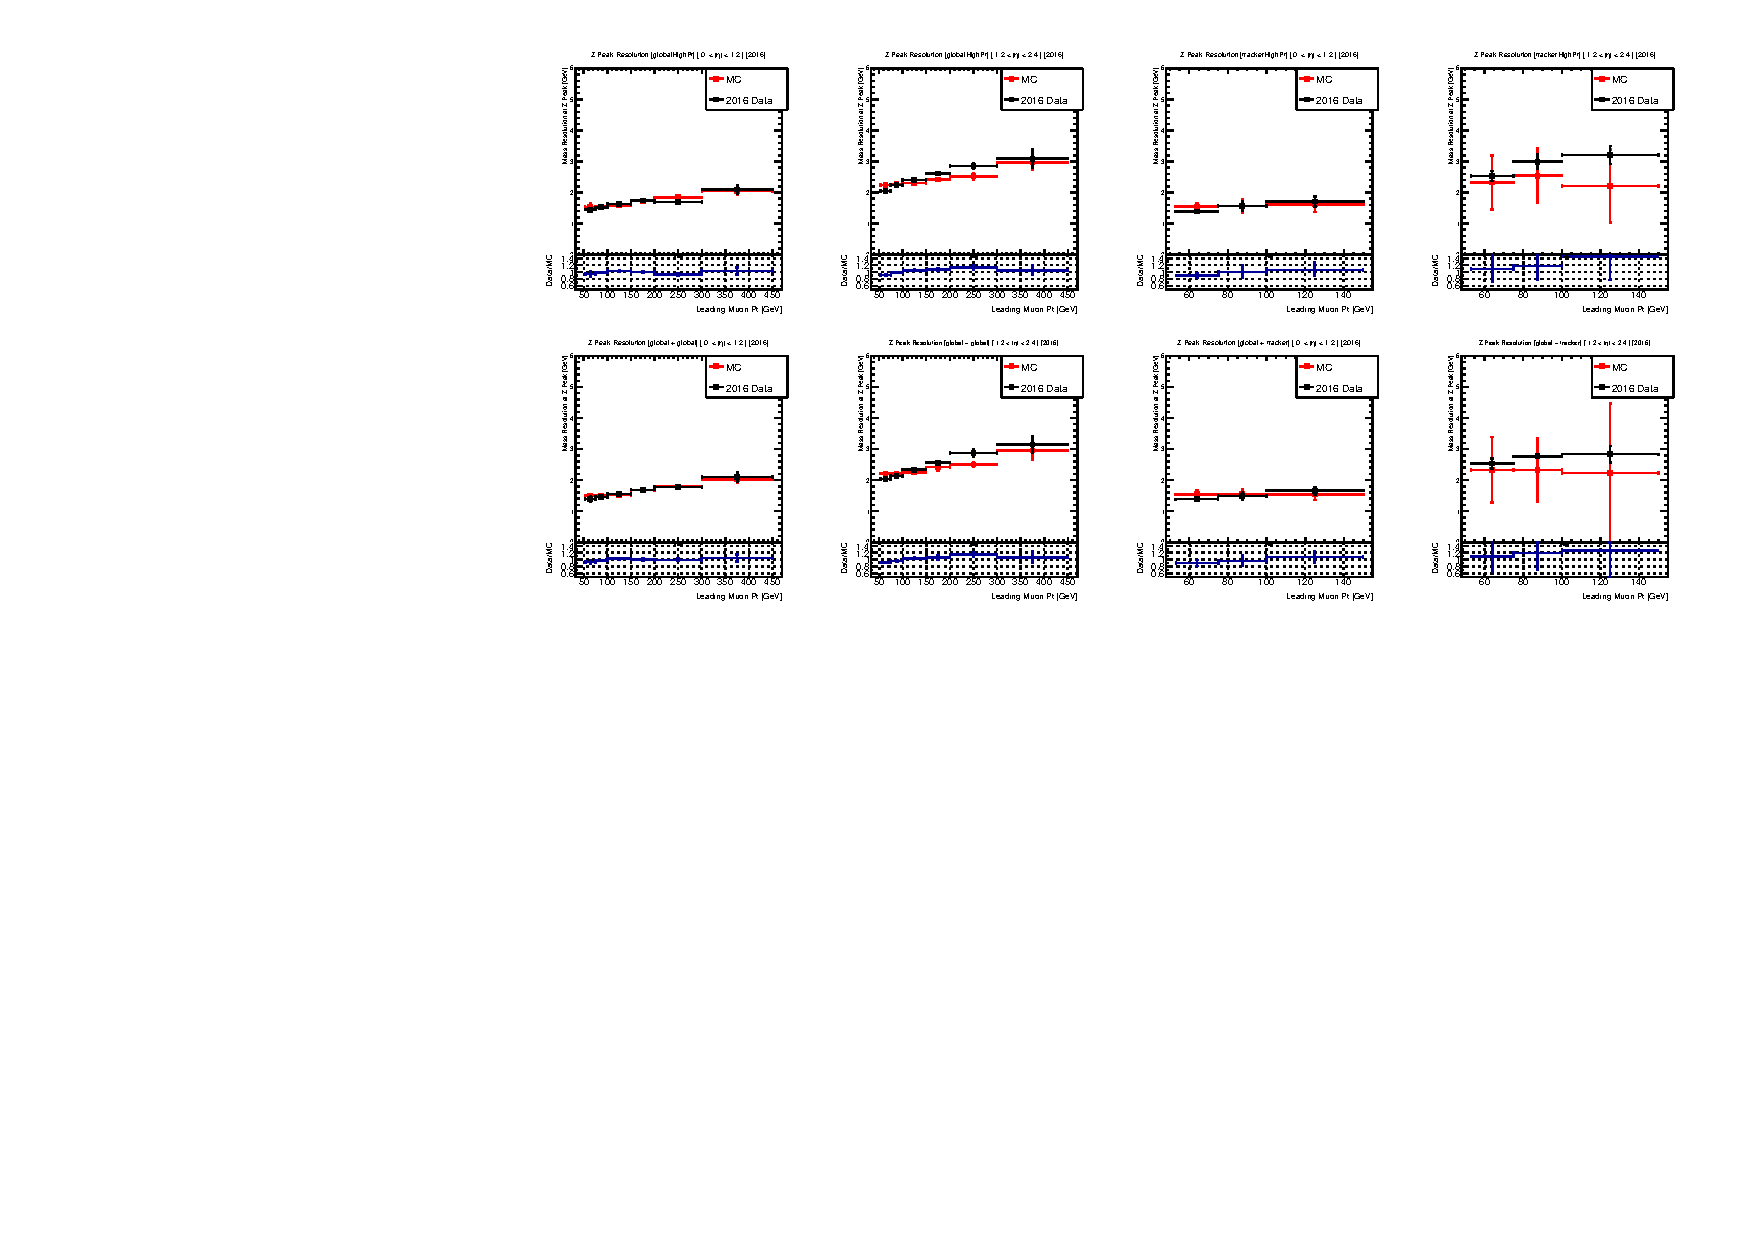
\includegraphics[width=.9\textwidth]{fig/MomentumResolution/2016_ZPeakResolution_Summary.pdf}
  \caption{Mass resolution at Z peak as a function of the leading muon's transverse
    momentum for the \texttt|global| and \texttt|trackerHighPt| found in the barrel and endcaps
    on the muon systems}
  \label{fig:ZMassResolution_Summary}
\end{figure}

The dimuon mass can be used to validate simulation in data, where the true momentum
of the muon is unknown. For this, a Data/MC comparisson is done over the
distributions for the reconstructed dimuon mass. The distributions are built
from the reconstructed mass as a function of the muon transverse momentum and
obtained for each individual muon. The mass resolution distribution is then fitted with
a Breit-Wigner convolution of the Double-Sided crystal ball, from this fit the
standard deviation of the gaussian portion of the DSCB equates the dimuon
mass resolution. Fits for data and montecarlo simulation are shown in figures
\ref{fig:ZMassResolution_Data_Global} and \ref{fig:ZMassResolution_MC_Global}
with the results from the fits and the Data/MC comparison is shown on figure
\ref{fig:ZMassResolution_Summary}.

